\subsection{Eure Profs}

\subsubsection{Algorithmen und Datenstrukturen}

\begin{figure}[h]
	\centering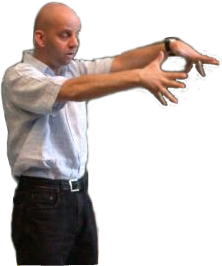
\includegraphics[width=0.7\linewidth]{bilder/dozenten/fekete_frei.png}\\
	{Prof. S\'andor Fekete}
\end{figure}
Diese Vorlesung vermittelt Programmiersprachenunabh"angige Konzepte wie B"aume, Listen oder Stacks. Wer nicht wei"s, was sich hinter diesen Begriffen verbirgt, sollte auf keinen Fall die "Ubungen verpassen.


\subsubsection{Diskrete Mathematik}

% \begin{figure}[h]
% 	\centering\includegraphics[width=0.7\linewidth]{bilder/kemnitz.png}\\
% 	{Dr. Arnfried Kemnitz}
% \end{figure}
Diskrete Mathematik handelt von allem, was mit ganzen Zahlen zu tun hat: Fibbonacci-Zahlen, Primzahlen, Modulorechnung, usw.


\subsubsection{Lineare Algebra}

\begin{figure}[h]
	\centering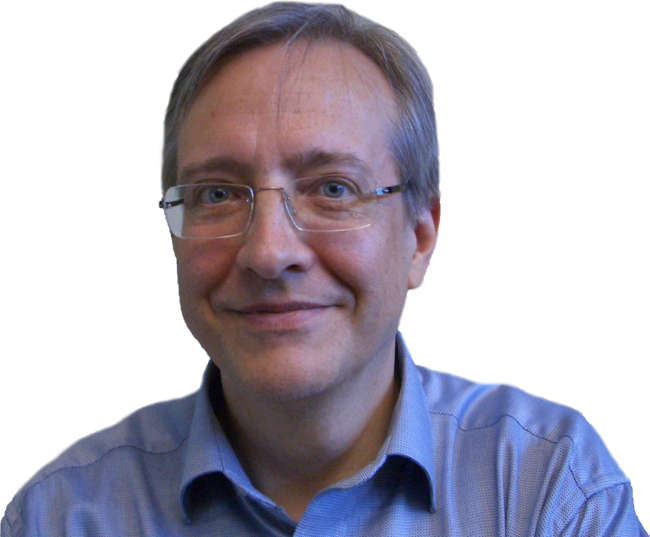
\includegraphics[width=0.7\linewidth]{bilder/dozenten/marten_frei.png}\\
	{Dr. Wolfgang Marten}
\end{figure}
Hier geht es um Vektoren und Matrizen, sowie ein wenig Gruppentheorie. Die
"Ubungen sind zwar nicht immer einfach, geben aber einen sehr guten Ausblick auf die Klausur.


\subsubsection{Programmieren 1}

\begin{figure}[h]
	\centering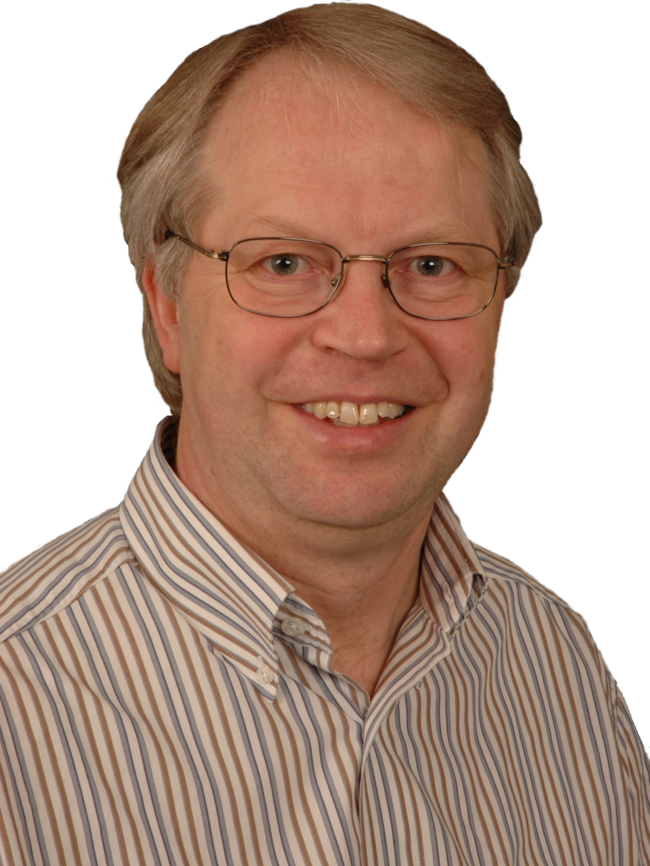
\includegraphics[width=0.7\linewidth]{bilder/dozenten/struck.png}\\
	{Dr. Werner Struckmann}
\end{figure}
Programmiert wird hier fast ausschlie"slich in Java. Wer keine oder nur wenig Erfahrungen mit Java gemacht hat, sollte unbedingt die kleinen "Ubungen bearbeiten.


\subsubsection{Wissenschaftliches Arbeiten}

% \begin{figure}[h]
% 	\centering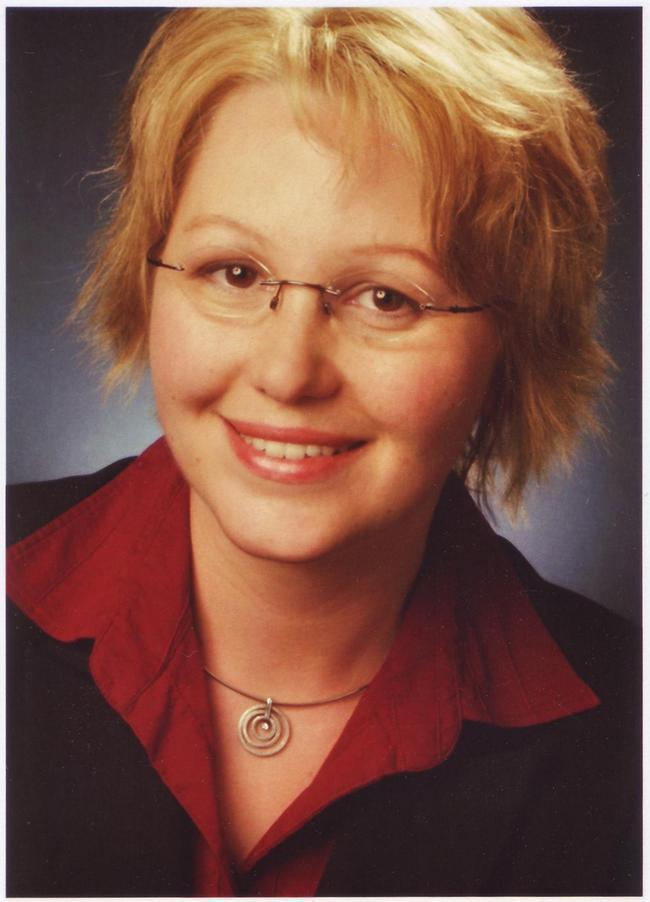
\includegraphics[width=0.7\linewidth]{bilder/dozenten/diethelm.png}\\
% 	{Dr. Ira Diethelm}
% \end{figure}
Hier werden Methoden und Richtlinien behandelt, die man zum Erstellen
wissenschaftlicher Arbeiten ben"otigt.
